A software tool named the ``kittingViewer'' is being developed that will
read files describing the initial state, the goal state, and the plan for
getting from the initial state to the goal state. The kittingViewer will
simulate execution of the plan, display a view of the plan being executed,
and produce and display metrics about the plan.  All of the metrics will be
numbers. All but one of the metrics will be objective and require no human
judgement. The final metric will be a subjective combination of the other
metrics in which the other metrics will be weighted and combined as desired
by the user.

The kittingViewer is partially built. It is able to read in the three
input files and simulate execution of the plan file. Plan metrics are
being calculated, and robot motion is being animated at speeds specified
in the plan.

Figure~\ref{fig:KittingViewer} shows the kittingViewer display at its
current state of development. The display uses three windows, labeled
Metrics \& Settings, Kitting Viewer, and Kitting Command. The windows may
be moved and resized independently, like other windows in a typical
windowing system. 

The Kitting Viewer window shows a view of the kitting workstation. The
floor of the workstation is covered with a grid. The spacing of the grid is
the last entry in the Metrics \& Settings window. The robot in the
workstation is represented by a gantry robot spanning the entire width of
the workstation.  The gantry robot moves when any of the CRCL motion
commands is executed.  The speed at which the picture of the robot is
animated matches the actual commanded speed of the robot.  When development
of the kittingViewer is complete, objects in the workstation will also be
shown (in color) and will move if the robot moves them.

The Kitting Command window shows the currently executing command or the
most recently executed command, if no command is currently executing.

The Metrics \& Settings window shows 9 metrics at the top and 14 settings
below that. All but three of the settings correspond to items that may be
set using CRCL commands. The extra three are the grid spacing and the robot
maximum speed and maximum acceleration (which may not be reset). As
commands are executed, metrics and settings are updated in the window.
When the kittingViewer is completed, there will be more metrics.
\begin{figure}[ht!]
\begin{center}
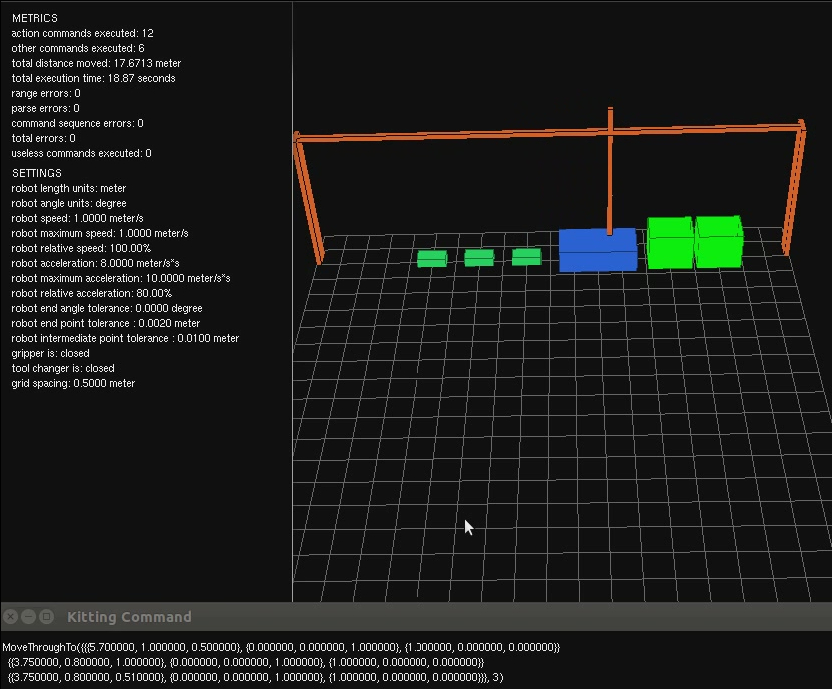
\includegraphics[width=8.5cm]{images/kittingViewer.jpg}
\caption{Kitting Viewer Display}
\label{fig:KittingViewer}
\end{center}
\end{figure}

\subsection{Errors}
In order to fully evaluate an input file, many planning errors are noted, but
ignored.
 If a range error
  occurs, an error message is printed in the terminal window from which the
  kittingViewer was started. The \sf SetRelativeAcceleration(-110) \rm
  command in Figure~\ref{fig:KittingPlan} causes two range errors, one
  because it is negative, and one because its absolute value is greater
  than 100.
  
  When the parser
  encounters a line that it cannot parse, it adds an \sf UnreadableMsg \rm to the
  list of commands it has parsed. The \sf UnreadableMsg \rm includes the text of
  the line on which the parse error occurred. When the \sf UnreadableMsg \rm is
  executed, the value of parse errors is increased by one and the
 \sf  UnreadableMsg \rm is displayed in the Kitting Command window so the user can
  see the line that caused the problem. The \sf MoveStraightTo(87) \rm
  command in Figure~\ref{fig:KittingPlan} causes a parse error.\\
  
\subsection{Controlling The Kitting Viewer}
Controlling the kittingViewer is accomplished by using the mouse and single
keys on the keyboard. When the kittingViewer starts up, a set of one-line
instructions is printed in the terminal window from which the
kittingViewer was started. Those instructions have the same meaning as
the longer explanations given below.\\

\begin{itemize}

\item \lq{}r\rq{} key -- the \lq{}r\rq{} key toggles the behavior of the left mouse button
  between translating and rotating the picture. This functionality is
  included because some mice do not have a middle button. Press R once and
  the left mouse button controls rotation. Press R again and the left
  mouse button controls translation (the original setting).\\

\item Left mouse button -- by default, the left mouse button is used to
  translate the picture. Position the cursor anywhere in the Kitting Viewer
  window, hold down the left mouse button and move the cursor by moving the
  mouse. The picture will move as though it is glued to the cursor. If the
  R key has switched the left mouse button to rotation, it behaves like the
  middle mouse button, as described in the next paragraph.\\

\item Middle mouse button -- the middle mouse button is used to rotate the
  picture. This is a little trickier than the other two mouse buttons. To
  rotate the picture, position the cursor inside the window near an edge of
  the window, hold down the middle mouse button, and move the cursor in a
  straight line towards the opposite edge. The picture rotates around an axis
  that is perpendicular to the line of mouse motion. In order
  to allow for fine positioning, the amount of rotation that occurs for a
  given amount of mouse motion decreases as the picture is zoomed
  in. Hence, if you want to turn the picture completely over, it is best to
  zoom out, rotate, and zoom back in again.\\

\item Right mouse button -- the right mouse button is used to zoom in or
  out. To zoom out, position the cursor near the bottom of the picture,
  hold down the right mouse button and push the mouse away from you (moving
  the cursor up); that appears to push the picture away from you. To zoom
  in, position the cursor near the top of the picture, hold down the right
  mouse button and pull the mouse toward you (moving the cursor down); that
  appears to pull the picture toward you. Moving the mouse side to side
  while holding down the right mouse button does nothing. There are limits
  to how far in or out you can zoom. At the highest magnification, it is
  easy to see a separation of half a millimeter. This is zooming, not
  moving the point of view, so the eye never goes through the picture.\\

\item \lq{}h\rq{} key -- if the \lq{}h\rq{} key is pressed, the view in the Kitting Viewer
  window returns to its original position.\\

\item \lq{}g\rq{} key -- if the \lq{}g\rq{} key is pressed when the plan is not completely
  executed and no action command is executing, the next command in the plan
  is executed and the Metrics \& Settings window is updated. If the g key
  is pressed when the plan is completely executed or when an action command
  is in progress, nothing happens.\\

\item \lq{}t\rq{} key -- if the \lq{}t\rq{} key is pressed, a combined image of all the windows
  will be saved in a file. The name of the file will be anaglyph\_N.ppm,
  where N starts at 0000 and increases by 1 each time the t key is
  pressed. The ppm (portable pixmap) format is a common graphics format
  that many graphics utilities can handle.\\

\item \lq{}z\rq{} or \lq{}q\rq{} key -- if the \lq{}z\rq{} or \lq{}q\rq{} key is pressed, the kittingViewer program
  exits, and the windows disappear.\\

\end{itemize}
